

%   \begin{figure*}[ht]
%     \centering
%      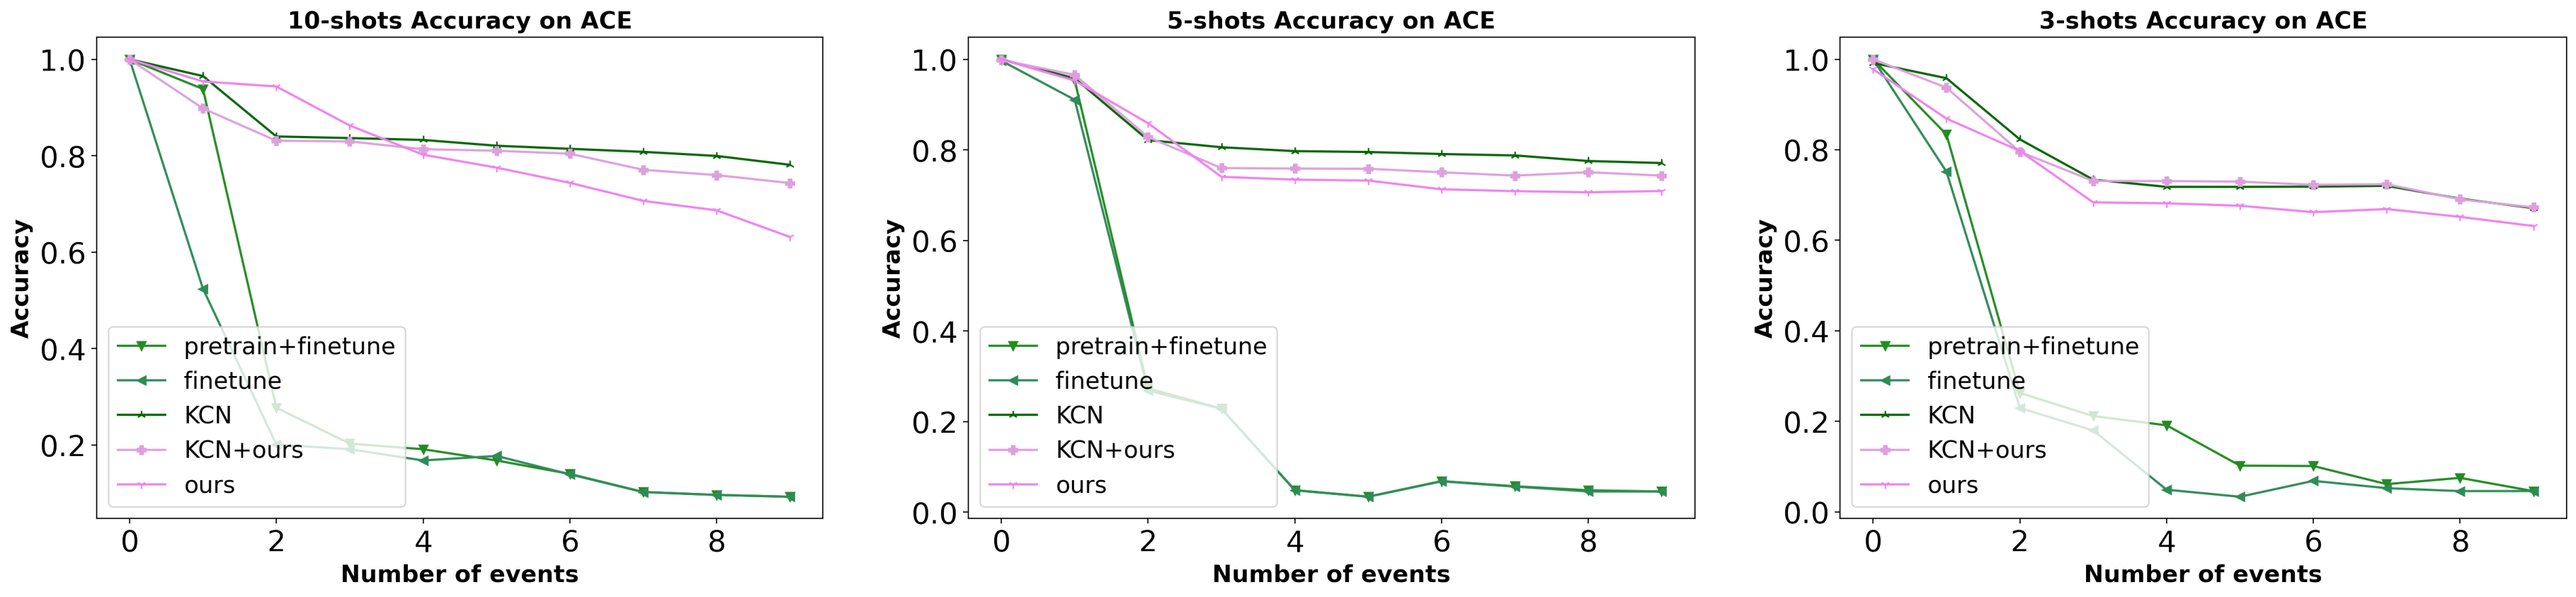
\includegraphics[width=\linewidth]{imgs/MAVEN_ACE.pdf}
%      \caption{10-shot, 5-shot, and 3-shot results using ACE05 as meta-testing set}
%      \label{fig:MAVEN_ACE}
%  \end{figure*}


  
\subsection{Dataset and Continual Few-shot Event Detection Task}
We adopted two widely used datasets for event detection and created the continual few-shot event detection tasks for evaluation. The dataset statistic are shown in Table~\ref{tab:stats}.

\noindent
\textbf{ACE 2005 English} \footnote{\url{https://catalog.ldc.upenn.edu/LDC2006T06}}: ACE 2005 English contains 33 event types.  To conduct our few-shot experiment, we filtered out events that have less than 10 interactions.

\noindent
\textbf{MAVEN} \citep{wang2020MAVEN}: MAVEN dataset contains 168 event types and are much more diverse compared to the ACE05 dataset. Each event type also has significantly more instances.  Due to limited computational resources, we choose to keep the top 50 event types by number of instances.  

\noindent
\textbf{Continual Few-shot Event Detection}: There is no available benchmark for continual few-shot event detection. Therefore, we propose the following construction method: for a given dataset,  we first construct a few-shot event detection dataset following a similar setup as \citep{chen2021honey}.  In particular,  for every event type,  we subsample its instances to simulate a few-shot condition.  For each event type, we randomly sample few instances as the support set, and the all other instances are used as the query set for evaluating.  For the continual event detection,  we followed the setup in \citep{cao2020incremental}.  We exploit the data of the top 10 most frequent event classes for continual learning. One new event class will be available for the model at each time, and we test the model on all previously seen event types. 

\begin{figure*}[ht]
\centering
    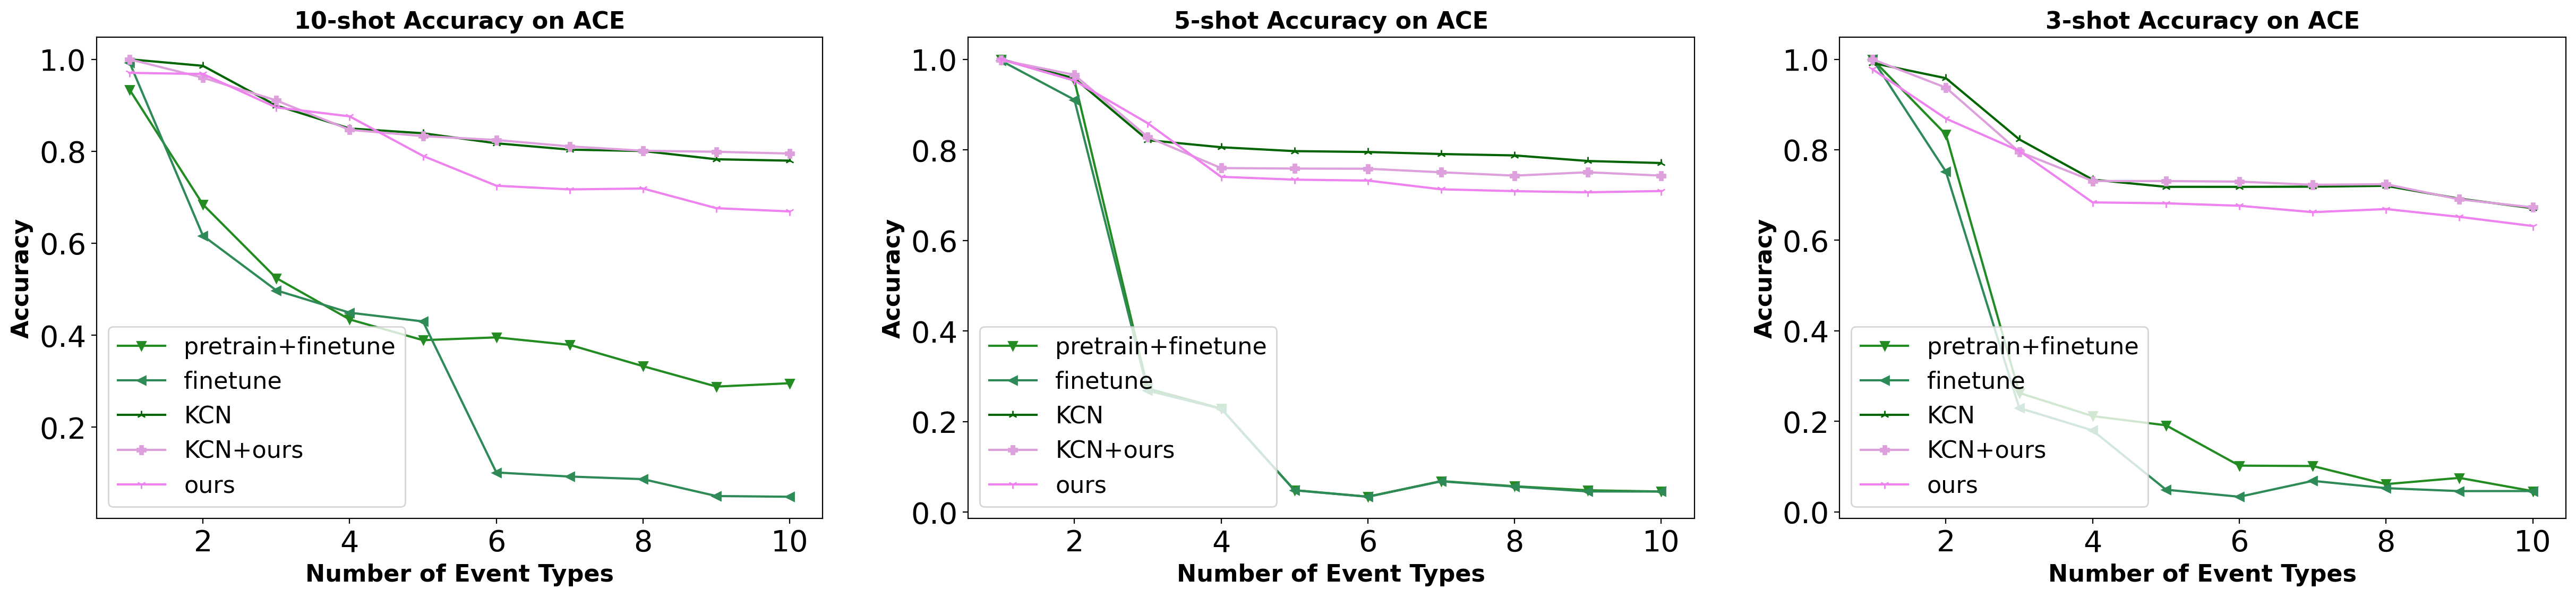
\includegraphics[scale=0.28]{imgs/MAVEN_ACE.jpg}
    \caption{10-shot, 5-shot, and 3-shot results using ACE05 as meta-testing set}
    \label{img:result_ACE}
\end{figure*}
\subsection{Meta-Training and Meta-Testing Detail}
\textbf{Meta-Training}: We used BERT \citep{devlin2018bert} as the representation module and a fully connected layer as the classifier.  In each training episode, we sample a continuous data trajectory of event instances.  The trajectory construction follows \ref{img:2}. 

\noindent
\textbf{Meta-Testing}: During the meta testing stage,  we followed the continual few-shot event detection setup. The support set for each event type comes in a class-incremental way. After each batch of support set arrives, we tested the model on all seen query sets. 

\subsection{Baselines}
We compare out approach with the following baselines: 

\noindent
\textbf{Finetune}: The model is simply fine-tuned whenever a stream of data arrives.

\noindent
\textbf{Pretrain + finetune}: We fine-tune the language model that are pretrained on the meta-training set. 

\noindent
\textbf{KCN}\citep{cao2020incremental}: KCN focuses on incremental event detection and uses prototype enhanced retrospection and hierarchical distillation to mitigate the adverse effects of semantic ambiguity and class imbalance. We initialized the language model used in KCN with a pretrained language model that is trained on the meta-training set to ensure a fair comparison. 

%We have not include the work by \cite{yu2021lifelong} 
We also implemented a model of  \cite{yu2021lifelong} following our experimental setup. However, this method could only reach an accuracy of ~0.4 while our method or KCN could reach ~0.7. There are some possible explanations for this result: 
\begin{enumerate}[noitemsep]
\item We might have some implementation errors of  \cite{yu2021lifelong} or a different configuration of hyper-parameters is required due to the new few-shot learning. For example, changing the default learning rate (1e-4)  in  \cite{yu2021lifelong}  to (6e-4) could help improve the final accuracy from ~0.1 to ~0.4. And some other hyper-parameters, i.e. the size of experience replay are also sensitive to the few-shot learning. We believe that a more concrete hyper-parameter search could further improve the performance. 

\item \cite{yu2021lifelong}  is not designed for a few-shot learning setting; there are thousands of  training data in the original experiments while there are only 10 training data in our setting. However, we believe that we could combine our model with his proposed method of knowledge distillation + knowledge transfer strategy. 

\item \cite{yu2021lifelong} adopts a different formulation of incremental event detection.
\end{enumerate}

We test our meta-learned representation for continual few-shot event detection by using it as the language model initialization for KCN. (KCN+ours), and adding a simple fully connected layer for fine-tuning(ours). 

\subsection{Experimental Setup}
While meta-testing on the ACE05 dataset, we used the MAVEN dataset as the meta-training set and vice versa.  We conducted our experiments in 10-shot, 5-shot and 3-shot settings.  We use accuracy as the evaluation metric. We choose a simple fully connected layer for the adaptation module.  All experiments were conducted on the HAL cluster \citep{HAL}. Our implementation has been submitted on Canvas. 

\subsection{Experimental Results}
As expected,  in Figure \ref{img:result_ACE} both the fine-tune and pretrain + finetune suffer from catastrophic interference. Their performance dropped significantly after 1 increment in event types. On the other hand, our meta-learned representation module with a simple fine-tune fully connected layer demonstrates strong performance across different few-shot setups.  However, it is not able to achieve the same level of performance as KCN and KCN + ours. Our speculation is that simply fine-tuning the model on the meta-learned representation module suffers from some degree of forgetting problem as it lacks the exmapler/memory set to store previous knowledge. Moreover, it cannot learn from previous examples as effectively as KCN since there is no distillation strategy. On the other hand KCN + ours outperforms KCN under the 10 shot setting, and is on par with KCN for 5-shot and 3-shot setup. 

\subsection{Case Study}
We also tested our representation module to see if it can be generalized to larger dataset.  We used ACE05 as the meta-training set and MAVEN as the meta testing set. 

\begin{figure}[h]
\centering
    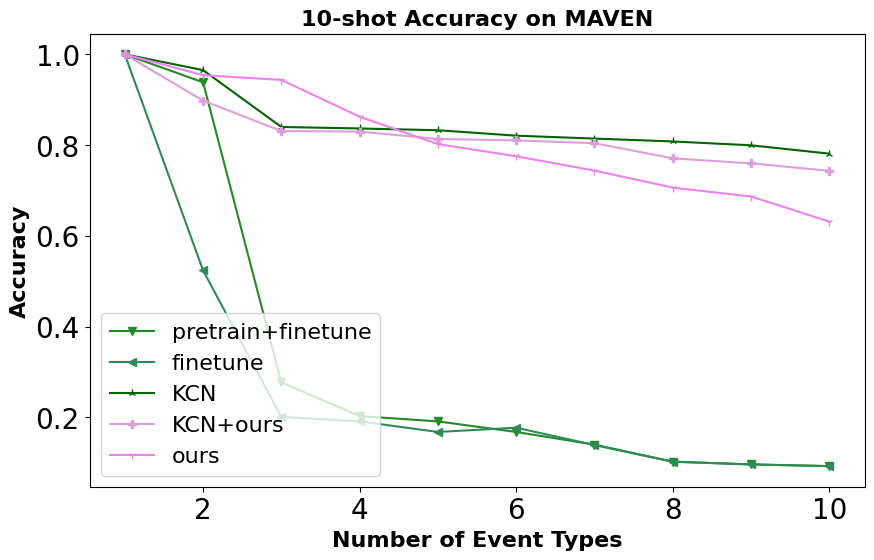
\includegraphics[scale=0.28]{imgs/ACE_MAVEN.jpg}
    \caption{10-shot results using MAVEN as meta-testing set}
    \label{img:result_MAVEN}
\end{figure}

As we can see,  both ours and KCN + ours have worse performance than KCN.  We suspect the issue is that MAVEN is a significantly larger and more diverse dataset compared to ACE05. Our meta-learned representation module might not generalize well enough to give robust performance on the continual few-shot event detection task.
